\section{Detección digital en presencia de ruido}

\begin{figure}[htb]
    \centering\begin{minipage}{\textwidth}
    \bpgf{Imagenes/detDig/detDig-1}
    \begin{blockdiagram}
        \matrix[row sep=5 mm, column sep=10mm]{
            & & & \node[punto] (p1) {}; & \node[etiqueta] (muestreo) {} node [anchor=south]{muestreo} ;\\
            \node [punto] (inicio) {} node [anchor=east] {$\sum_k a_k p(t-kT_s) + n(t)$}; & \node [punto] (p2) {}; &\node [punto] (p3) {}; & &\node [punto] (p4) {} node [anchor=north] {$y$}; &\node [block] (comp) {COMP}; &\node [etiqueta] (salida) {$\hat{a}_k$}; \\
            & & \node [block] (sinc) {SINCR}; & \node [punto] (p5) {};\\
        };
        \draw (inicio) -- (p2) -- (p3) -- (muestreo);
        \draw [->] (p2) |- (sinc);
        \draw (sinc) -- (p5);
        \draw [->,dashed] (p5) -- (p1);
        \draw [->] (p4) -- (comp);
        \draw [->] (comp) -- (salida);
    \end{blockdiagram}
    \endpgfgraphicnamed\end{minipage}
\end{figure}
\FloatBarrier

Recibo la onda digital de banda base contaminada de ruido. Suponemos por ahora:
\begin{itemize}
    \item Sincronización perfecta.
    \item No hay ISI. O sea que los pulsos son de Nyquist o que tengo ancho de banda suficiente para que pasen pulsos rectangulares sin distorsión apreciable.
    \item A la entrada del comparador, tenemos la muestra $y_k = a_k + n_k$, donde \\
%\begin{itemize}
%\item $a_k$ es el símbolo transmitido.%una muestra de ruido
%\item $n_k$ es una muestra de ruido
%\end{itemize}
$\begin{cases}
a_k \in \mathcal{A} & \text{ es el símbolo transmitido}\\
n_k=n(kT_s) & \text{ es una muestra de ruido}
\end{cases}$.
\end{itemize}

Suponemos que $n_k$ tiene $E[n_k]=0$, $E[n_k^2]=\sigma^2$, y
densidad de probabilidad $f_N(n)$.

\begin{minipage}{0.5\textwidth}
    \bpgf{Imagenes/detDig/detDig-2}
    \begin{tikzpicture}
        \draw [->] (-3,0) -- (3,0) node [anchor=north] {$n$};
        \draw [->] (0,-0.5) -- (0,2.5) node [anchor=west] {$f_N(n)$};
        \draw [domain=-2.5:2.5,samples=200] plot (\x,{2*exp(-1*((\x)^2))});
    \end{tikzpicture}
    \endpgfgraphicnamed
\end{minipage}
\begin{minipage}{0.5\textwidth}
\[\int_a^b f_N(n)\d n = Prob (a\leq n_k \leq b).\]
\end{minipage}

Por ahora no entramos en el tema de cómo el ruido $n(t)$ se generó
en el canal analógico. Típicamente, será un ruido blanco que se
filtra en recepción. Postergamos ese análisis.

\subsection*{Probabilidad de error de detección, s\'imbolos binarios}

Consideramos primero el caso binario, donde $a_k$ toma dos valores
posibles, $A_1 < A_2$. \\ Por ejemplo: $A_1=0, A_2 = A$ en el caso
unipolar.

La densidad de probabilidad de la V.A. $Y$ recibida, es la de $n$
trasladada por el símbolo. Tenemos por tanto $2$ densidades
\emph{condicionales} al símbolo enviado,
\begin{gather*}
    f_{Y|A_1} (y) = f_N(y-A_1);\\
    f_{Y|A_2} (y) = f_N(y-A_2).
\end{gather*}

\begin{figure}[htb]
    \centering\begin{minipage}{\textwidth}
    \bpgf{Imagenes/detDig/detDig-3}
    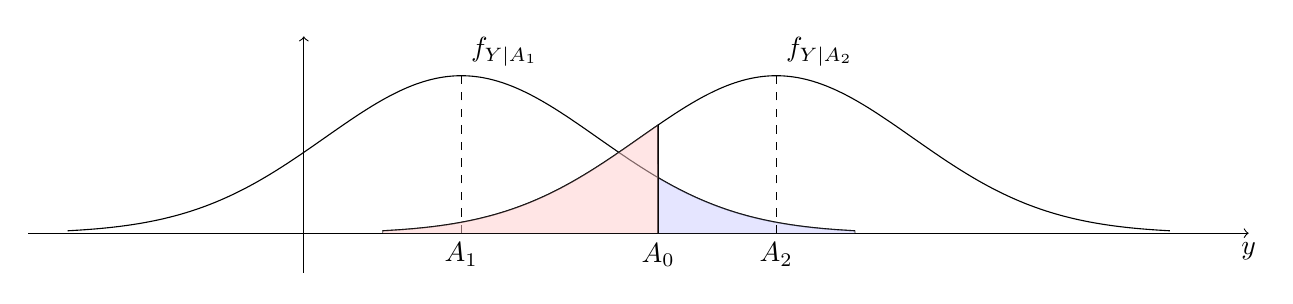
\begin{tikzpicture}
        \draw [->] (-3.5,0) -- (12,0) node [anchor=north] {$y$};
        \draw [->] (0,-0.5) -- (0,2.5);
        \draw [domain=-3:7,samples=200] plot (\x,{2*exp(-1*((\x-2)^2)/6)});
        \draw [dashed] (2,0) node [anchor=north] {$A_1$} -- (2,2) node [anchor=south west] {$f_{Y|A_1}$};
        \draw [domain=4.5:7,samples=200,fill=blue!20,opacity=0.5] (4.5,0) --  plot (\x,{2*exp(-1*((\x-2)^2)/6)}) -- (7,0);
        \begin{scope}[shift={(4,0)}]
            \draw [domain=-3:7,samples=200] plot (\x,{2*exp(-1*((\x-2)^2)/6)});
            \draw [dashed] (2,0) node [anchor=north] {$A_2$} -- (2,2) node [anchor=south west] {$f_{Y|A_2}$};
            \draw [thick] (0.5,0) node [anchor=north] {$A_0$} -- (0.5,{2*exp(-1*(1.5^2)/6)});
            \draw [domain=-3:0.5,samples=200,fill=red!20,opacity=0.5] (-3,0) --  plot (\x,{2*exp(-1*((\x-2)^2)/6)}) -- (0.5,0);
        \end{scope}
    \end{tikzpicture}
    \endpgfgraphicnamed\end{minipage}
\end{figure}
\FloatBarrier

Decidimos si se transmitió $A_1$ o $A_2$ comparando con un umbral
$A_0$. Entonces hay un error de detección si:
\begin{itemize}
    \item $y>A_0$ y se transmitió $A_1$;
    \item $y<A_0$ y  se transmitió $A_2$.
\end{itemize}

Calculo la probabilidad de cada evento, indicada en sombreado.
\begin{align*}
    P(\text{error}|A_1) &= \int_{A_0}^\infty f_N(y-A_1)\d y = \int_{A_0-A_1}^\infty f_N(n)\d n;\\
    P(\text{error}|A_2) &= \int_{-\infty}^{A_0} f_N(y-A_2)\d y = \int_{-\infty}^{-(A_2-A_0)} f_N(n)\d n.\\
\end{align*}

\begin{figure}[htb]
    \centering\begin{minipage}{\textwidth}
    \bpgf{Imagenes/detDig/detDig-4}
    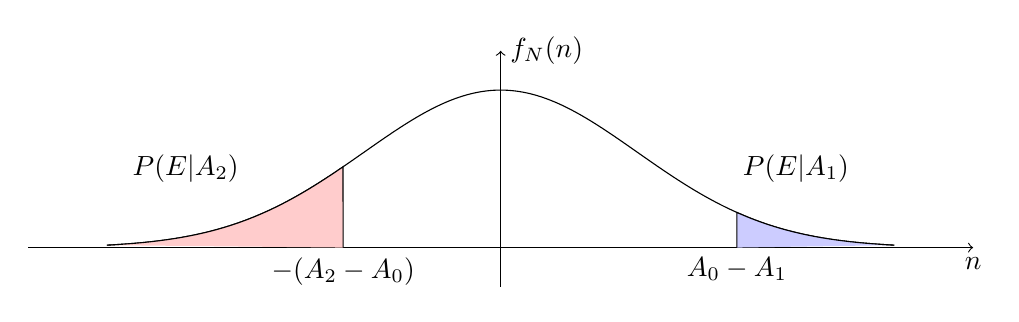
\begin{tikzpicture}
        \draw [->] (-6,0) -- (6,0) node [anchor=north] {$n$};
        \draw [->] (0,-0.5) -- (0,2.5) node [anchor=west] {$f_N(n)$};
        \draw [domain=-5:5,samples=200] plot (\x,{2*exp(-1*((\x)^2)/6)});
        \draw [domain=-5:-2,samples=200,fill=red!20] plot (\x,{2*exp(-1*((\x)^2)/6)}) -- (-2,0) node [anchor=north] {$-(A_2-A_0)$};
        \draw [domain=3:5,samples=200,fill=blue!20] (3,0) node [anchor=north] {$A_0-A_1$} -- plot (\x,{2*exp(-1*((\x)^2)/6)});
        \path (-4,1) node {$P(E|A_2)$};
        \path (3.75,1) node {$P(E|A_1)$};
    \end{tikzpicture}
    \endpgfgraphicnamed\end{minipage}
\end{figure}
\FloatBarrier

Esas son probabilidades condicionales. La probabilidad total es:
\[P_e = P(E|A_1) P (A_1) + P(E|A_2) P (A_2).\]

\subsubsection*{Umbral óptimo}

Si subimos el umbral $A_0$, $P(E|A_1)$ baja pero sube $P(E|A_2)$,
y viceversa. Entonces hay un compromiso en la elección del umbral.
La selección óptima es la que minimiza $P_e$; la hallamos por
diferenciación.

\[\frac{\partial P_e}{\partial A_0} = P(A_2) f_N(A_0 - A_2) - P(A_1) f_N (A_0 - A_1).\]

Existe $A_0^*$ que anula la derivada, que cumple
\[\frac{P(A_2)}{P(A_1)}=\frac{f_N(A_0^*-A_1)}{f_N(A_0^*-A_2)}.\]

\subsubsection*{Caso usual: símbolos equiprobables, ruido simétrico}

$P(A_1) = P(A_2) = \frac{1}{2}\Rightarrow f_N(A_0^*-A_1) =
f_N(A_0^*-A_2)$.

Supongamos $f_N(n)$ simétrica (par) y decreciente en $n>0$ (caso típico: Gaussiana).

\begin{figure}[htb]
    \centering\begin{minipage}{\textwidth}
    \bpgf{Imagenes/detDig/detDig-5}
    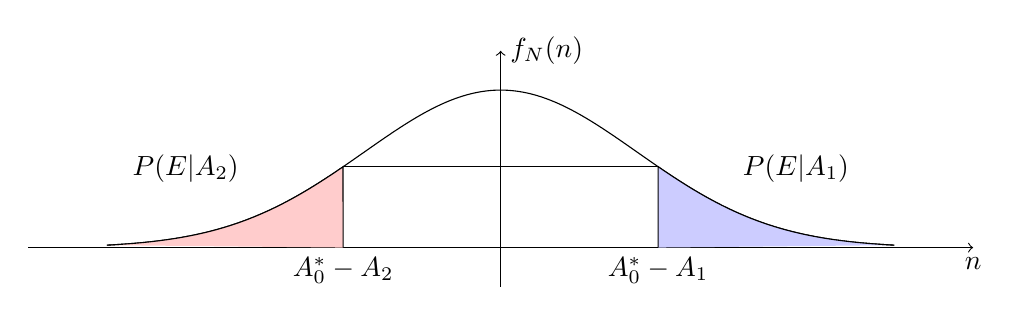
\begin{tikzpicture}
        \draw [->] (-6,0) -- (6,0) node [anchor=north] {$n$};
        \draw [->] (0,-0.5) -- (0,2.5) node [anchor=west] {$f_N(n)$};
        \draw [domain=-5:5,samples=200] plot (\x,{2*exp(-1*((\x)^2)/6)});
        \draw [domain=-5:-2,samples=200,fill=red!20] plot (\x,{2*exp(-1*((\x)^2)/6)}) -- (-2,0) node [anchor=north] {$A_0^*-A_2$};
        \draw [domain=2:5,samples=200,fill=blue!20] (2,0) node [anchor=north] {$A_0^*-A_1$} -- plot (\x,{2*exp(-1*((\x)^2)/6)});
        \path (-4,1) node {$P(E|A_2)$};
        \path (3.75,1) node {$P(E|A_1)$};
        \draw (2,{2*exp(-2/3)}) -- (-2,{2*exp(-2/3)});
    \end{tikzpicture}
    \endpgfgraphicnamed\end{minipage}
\end{figure}

Para que sean iguales las $f_N$, $A_2-A_0^* = A_0^*-A_1
\Rightarrow A_0^*=\dfrac{A_1+A_2}{2}$. \\
También $P(E|A_1) =
P(E|A_2)$. En este caso:
\[
{\col{P_e= P(E|A_1) = P(E|A_2) = \int_{\frac{A_2-A_1}{2}}^\infty
f_N(n)\d n}}
\]
Si en cambio, $P(A_2) > P(A_1)$ por ejemplo, entonces
$f_N(A_0^*-A_1) > f_N(A_0^*-A_2) \Rightarrow A_0^*-A_1 <
A_2-A_0^*$. El umbral óptimo está más cerca del símbolo menos
probable.

\subsection*{Probabilidad de error óptima, binario, ruido Gaussiano}
El modelo más usado para la distribución de probabilidad del ruido
es la normal o Gaussiana:
\[f_N(n) = \frac{1}{\sqrt{2\pi}\sigma}\e^{-\frac{n^2}{2\sigma^2}}\qquad \text{ (media $0$, varianza $\sigma^2$)}.\]
Denotamos por $Q(z)$ la probabilidad de que una normal standard
($\sigma=1$) supere a $z$,
\[Q(z):=\frac{1}{\sqrt{2\pi}} \int_z^\infty \e^{-\frac{n^2}{2}}\d n.\]
\begin{itemize}
    \item No tiene expresión analítica, pero está tabulada.
    \item Para $z \gg 1$, vale la aproximación $Q(z)\approx
    \frac{1}{\sqrt{2\pi}z}\e^{-\frac{z^2}{2}}$.
\end{itemize}

Si tengo un ruido $n$ normal $(0,\sigma^2)$, entonces $\frac{n}{\sigma}$ tiene varianza $1$. Por tanto,
\[P(n>z) = P \left(\frac{n}{\sigma}>\frac{z}{\sigma}\right) = Q\left(\frac{z}{\sigma}\right).\]

Entonces, para la detección con símbolos binarios equiprobables,
ruido Gaussiano $(0,\sigma^2)$, llegamos a la siguiente fórmula
para la probabilidad de error:
\[P_e=\int_{\frac{A_2-A_1}{2}}^\infty f_N(n)\d n = P\left(n>\frac{A_2-A_1}{2}\right) = Q\left(\frac{A_2-A_1}{2\sigma}\right).\]

\begin{ejemplo}[binario, equiprobable, ruido Gaussiano]$\phantom{1}$
\begin{description}
    \item[Unipolar] $A_1=0$, $A_2=A$, $A_0^* = \frac{A}{2}$,
    $P_e=Q\left(\frac{A}{2\sigma}\right)$.
    \item[Polar] $A_1=-A$, $A_2=A$, $A_0^* = 0$, $P_e =
    Q\left(\frac{A}{\sigma}\right)$.
 \end{description}
Notar que en ambos casos, para reducir $P_e$, debo aumentar
$\frac{A}{\sigma}$. De hecho, $P_e$ cae muy rápidamente:
%\begin{remarkSN}$\phantom{1}$
%    \begin{itemize}
%        \item Para achicar  \\
        \begin{center}
            \begin{tabular}{c|c}
                $\frac{A}{\sigma}$ & $Q\left(\frac{A}{\sigma}\right)=P_e(\text{polar})$\\
                \hline
                $2$ & $0.022$\\
                $4$ & $3\cdot 10^{-5}$\\
                $6$ & $10^{-8}$
            \end{tabular}
        \end{center}
\end{ejemplo}
%
%        Cae muy
%        \item
%    \end{itemize}
%\end{remarkSN}
$\frac{A}{\sigma}$ opera como una relación señal - ruido. De
hecho, $\sigma^2=E[n_k^2]=N$, potencia media de ruido. $A^2$ está
relacionado con la potencia de la onda $x(t) = \sum a_k
p(t-kT_s)$. La relación exacta depende de $p(t)$ y el código de
línea, veamos ejemplos.


\begin{ejemplo}
    $p(t)= p_{[0,T_s]}(t)$ NRZ. En este caso, vimos que $\langle x^2 \rangle = E[a_k^2]\frac{\|p\|^2}{T_s} =
    E[a_k^2]$. Casos particulares:
    \begin{align*}
    \text{Polar, NRZ: } \langle x^2 \rangle  &= A^2 \Rightarrow \left(\frac{S}{N}\right) = \frac{A^2}{\sigma^2}.\\
    \text{Unipolar,NRZ: } \langle x^2 \rangle &=\frac{A^2}{2}\Rightarrow \left(\frac{S}{N}\right) =
    \frac{A^2}{2\sigma^2}.
\end{align*}
    \begin{equation*}
        \Rightarrow \left.\begin{aligned}
                        P_e = Q\left(\sqrt{\frac{S}{N}}\right)\qquad &\text{polar}\\
                        P_e = Q\left(\frac{1}{\sqrt{2}}\sqrt{\frac{S}{N}}\right)\qquad &\text{unipolar}
                    \end{aligned} \right\rbrace
                    \text{\begin{minipage}{5cm}
                            polar es más eficiente: menor $P_e$ para igual
                            $\frac{S}{N}$.
                          \end{minipage}}
    \end{equation*}
\end{ejemplo}

\subsection*{Caso M-ario ($M$ símbolos por pulso)}

Elegimos una ``constelación'' de niveles para representar los $M$ símbolos. Por ejemplo, para $M$ par, elegimos una constelación polar $\{\pm A, \pm 3A,\pm 5A,\ldots\}$. El espaciamiento es $2A$. El nivel más grande es $(M-1)A$. Tomamos símbolos equiprobables y contaminamos con ruido Gaussiano, tenemos:

\begin{figure}[htb]
    \centering\begin{minipage}{\textwidth}
    \bpgf{Imagenes/detDig/detDig-6}
    {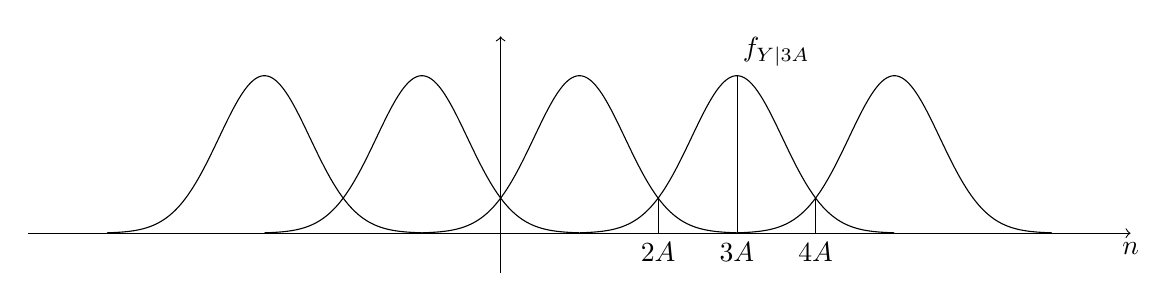
\begin{tikzpicture}
        \draw [->] (-6,0) -- (8,0) node [anchor=north] {$n$};
        \draw [->] (0,-0.5) -- (0,2.5);
        \foreach \a in {-3,-1,1,3,5}
            \draw [domain={\a-2}:{\a+2},samples=200] plot (\x,{2*exp(-1.5*((\x-\a)^2))});
        \path (3.5,2) node [anchor=south] {$f_{Y|3A}$};
        \draw [ultra thin] (2,0) node [anchor=north] {$2A$} -- (2,{2*exp(-1.5)});
        \draw [ultra thin] (4,0) node [anchor=north] {$4A$} -- (4,{2*exp(-1.5)});
        \draw [ultra thin] (3,0) node [anchor=north] {$3A$} -- (3,2);
    \end{tikzpicture}}
    \endpgfgraphicnamed\end{minipage}
\end{figure}
\FloatBarrier

Es intuitivo que los umbrales de detección óptimos son los puntos medios $0,\pm 2A, \pm 4A,\ldots$

Para cualquier símbolo menos los extremos
\[P(E|\text{simb}) = P(|n|>A) = 2P(n>A) = 2Q\left(\frac{A}{\sigma}\right).\]
Para los extremos
\[P(E|\text{simb}) = Q\left(\frac{A}{\sigma}\right).\]

\paragraph{TOTAL}

\[P_e=\frac{(M-2) 2 Q\left(\frac{A}{\sigma}\right) + 2Q\left(\frac{A}{\sigma}\right)}{M} = \underbrace{2\left(\frac{M-1}{M}\right)Q\left(\frac{A}{\sigma}\right)}_{\text{prob. error de símbolo}}.\]

Si queremos relacionar $P_e$ con $\left(\frac{S}{N}\right)$, otra
vez jugaría la forma de los pulsos.

\begin{ejemplo}
    Pulsos NRZ, $a_k$ polar M-ario.
    \[\langle x^2\rangle=E[a_k^2]=A^2\frac{2}{M}\left(1+3^2+5^2+\cdots+(M-1)^2\right) = \frac{2A^2}{M}\left(\frac{M^3-M}{6}\right) = \frac{A^2(M^2-1)}{3}\]

  Se utilizó arriba una fórmula para la suma de los cuadrados de los números
  impares, demostrable por inducción completa.

\[\Rightarrow \left(\frac{S}{N}\right)=\frac{A^2}{\sigma^2}\left(\frac{M^2-1}{3}\right) \qquad
\Rightarrow
{\col{P_e=2\left(\frac{M-1}{M}\right)Q\left(\sqrt{\frac{3}{M^2-1}\left(\frac{S}{N}\right)}\right)}}\]

    es menos eficiente que $M=2$, a cambio de más bps.
\end{ejemplo}

\subsubsection*{$P_e$ (símbolo) vs. $P_e$ (bit)}

En M-ario, un símbolo codifica $\log_2(M)$ bits. Si cometo un error de símbolo, me afecta varios bits, dependiendo de la correspondencia bits/símbolo.

\subsubsection*{Código de Gray} Símbolos vecinos difieren en $1$ sólo bit. Por ejemplo, para $M=8$

\begin{tabular}{r|r}
    $7A$ & $010$\\
    $5A$ & $011$\\
    $3A$ & $001$\\
    $A$  & $000$\\
    \hline
    $-A$ & $100$\\
    $-3A$ & $101$\\
    $-5A$ & $111$\\
    $-7A$ & $110$
\end{tabular} Despreciando la probabilidad de un salto de más de un nivel, tenemos aquí
\[P_e\text{(bit)} \approx \frac{P_e\text{(símb)}}{\log_2 M}.\]

\paragraph{Resumen (detección digital)}$\phantom{1}$

\FloatBarrier
\begin{figure}[htb]
    \centering\begin{minipage}{\textwidth}
    \bpgf{Imagenes/detDig/detDig-7}
    \begin{blockdiagram}
        \matrix[row sep=5 mm, column sep=10mm]{
            & & & \node[punto] (p1) {}; & \node[etiqueta] (muestreo) {} node [anchor=south]{muestreo} ;\\
            \node [punto] (inicio) {} node [anchor=east] {$\sum_k a_k p(t-kT_s) + n(t)$}; & \node [punto] (p2) {}; &\node [punto] (p3) {}; & &\node [punto] (p4) {} node [anchor=north] {$y_k=a_k+n_k$}; &\node [block] (comp) {COMP}; &\node [etiqueta] (salida) {$\hat{a}_k$}; \\
            & & \node [block] (sinc) {SINCR}; & \node [punto] (p5) {};\\
        };
        \draw (inicio) -- (p2) -- (p3) -- (muestreo);
        \draw [->] (p2) |- (sinc);
        \draw (sinc) -- (p5);
        \draw [->,dashed] (p5) -- (p1);
        \draw [->] (p4) -- (comp);
        \draw [->] (comp) -- (salida);
    \end{blockdiagram}
    \endpgfgraphicnamed\end{minipage}
\end{figure}
\FloatBarrier

\begin{itemize}
    \item pulsos sin ISI
    \item $\{a_k\} \in \mathcal{A}$ constelación de múltiplos de $A$. \\ Ejemplos: (i)
    $\mathcal{A} = \{-A, A\}$; (ii) $\mathcal{A} = \{0,A\}$; (iii)
    $\mathcal{A}= \{\pm A,\pm 3A,\ldots \}$. %
%    \begin{enumerate}
%        \item $\pm A$
%        \item $$
%        \item $\pm A,
%    \end{enumerate}
    \item Ruido $n(t)$, $E[n]=0$, $E[n^2]=\sigma^2$. Densidad $f_N(n)$. Por defecto, Gaussiano.
\end{itemize}

Decido mediante comparación de la muestra $y_k = a_k + n_k$, con
umbrales apropiados. $P_e$ es la probabilidad de error del símbolo
detectado.

Obtuvimos expresiones de $P_e$ en función de $\frac{A}{\sigma}$, para cada tipo de señalización.
 \begin{itemize}
        \item Polar, binario:
        $P_e=Q\left(\frac{A}{\sigma}\right)$.
        \item Unipolar: $P_e=Q\left(\frac{A}{2\sigma}\right)$.
        \item Polar, M-ario:
        $P_e\text{(simb)}=2\left(\frac{M-1}{M}\right)Q\left(\frac{A}{\sigma}\right)$.
    \end{itemize}

Para algunas formas de pulsos específicas, relacionamos
$\frac{A}{\sigma}$ con $\sqrt{\left(\frac{S}{N}\right)}$.
